\documentclass[journal]{IEEEtran}
\usepackage{amsmath,graphicx,Geoff,subfig,cite}

% Title.
% ------
\title{A Graph-Based Approach for Feature Extraction and Segmentation of Multimodal Images}
% 
% Single address.
% ---------------

\author{Geoffrey~Iyer,~Jocelyn~Chanussot,~\emph{Fellow, IEEE},~and~Andrea~L.~Bertozzi~\emph{Fellow, IEEE}% <-this % stops a space
}

% \author{Geoffrey Iyer$^1$, Jocelyn Chanussot$^{1,2,3}$, Andrea L. Bertozzi$^{1}$}
% \address{1. University of California, Los Angeles \\2. Univ. Grenoble Alpes, CNRS, GIPSA-lab, F-38000 Grenoble, France  \\3. Faculty of Electrical and Computer Engineering, University of Iceland, 101 Reykjavik, Iceland }

\begin{document}
% 
\maketitle
% 
\begin{abstract}
  In the past few years, graph-based methods have proven to be a useful tool in
  a wide variety of energy minimization problems.  In this paper, we propose a
  graph-based algorithm for feature extraction and segmentation of multimodal
  images. By defining a notion of similarity that integrates information from
  each modality, we create a fused graph that merges the different data sources.
  %%%% CUT: All the stuff about data level or feature level
  % By defining a notion of similarity that integrates
  % information from each modality, we merge the different sources at the data
  % level.
  %%%%%%%%%%%%%%%%%%%
  The graph Laplacian then allows us to perform feature extraction and
  segmentation on the fused dataset. We apply this method in a practical
  example, namely the segmentation of optical and lidar images. The results
  obtained confirm the potential of the proposed method.
  % By constructing a graph, we integrate the different information
  % sources at
  % the data level, producing a feature space that fuses the modalities
  % into one
  % coherent structure.
  % By creating a notion of distance in multimodal sets that preserves the
  % independent information in each modality, and integrating the
  % different sets
  % at the data level, we achieve more accurate segresults than
\end{abstract}

% \begin{keywords} Image segmentation, multimodal image, data fusion, graph
%   Laplacian, Nystr\"{o}m extension, graph cut minimization
% \end{keywords}

\section{Introduction}
\label{sec:intro}

With the increasing availability of data we often come upon multiple datasets,
derived from different sensors, that describe the same object or phenomenon. We
call the sensors \emph{modalities}, and because each modality represents some
new degrees of freedom, it is generally desirable to use more modalities rather
than fewer. For example, in the area of speech recognition, integrating audio
data with a video of the speaker results in a much more accurate classification
\cite{Potamianos03, sedighin:hal-01400542}. Similarly, in medicine, it is
possible to fuse the results of two different types of brain imaging to create a
final image with better resolution than either of the originals
\cite{Lei12,Samadi2016} .  In this paper we also focus on multimodal images, but
rather than seeking to merge our images, we instead perform feature extraction,
with applications toward segmentation.

In figure \ref{fig:DFCfig1} we show an example multimodal dataset from the 2015
IEEE Data Fusion Contest \cite{7536139} (abbreviated as DFC), which consists of
an optical and a lidar (elevation) image of a residential neighborhood in
Belgium. This particular dataset is interesting because of the large amount of
non-redundancy between the two images. By using the lidar data, one can easily
differentiate the roofs of the buildings from the adjacent streets, even though
they are roughly the same color. Conversely, the optical data allows one to
separate the many different objects at ground-level, even though they appear the
same in the lidar modality. Therefore one would expect that an algorithm that
processes the two sources together would produce much more accurate segmentation
results than could be obtained by dealing with the modalities separately.  We
will revisit this dataset in section \ref{sec:experiment} to show that this is
indeed the case.

\begin{figure*}[!t]
  \centering \subfloat[DFC optical
  data]{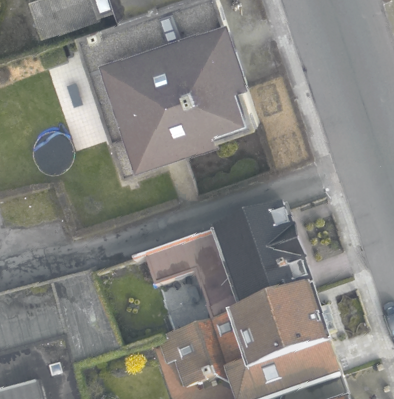
\includegraphics[width=2.5in]{./Images/DFC2015/optical.png}%
    \label{fig:DFCoptical}}%
  \hfil %
  \subfloat[DFC lidar
  data]{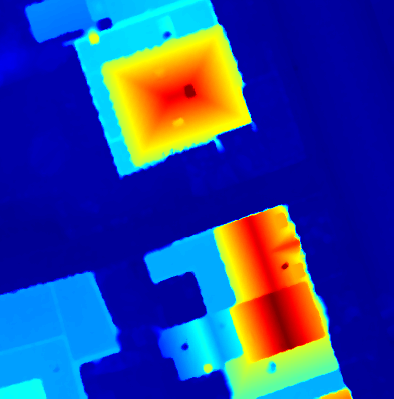
\includegraphics[width=2.5in]{./Images/DFC2015/lidarColor.png}
    \label{fig:DFClidar}} %
  \caption{DFC Input Data}
  \label{fig:DFCfig1}
\end{figure*}

% %%% An old paragraph. I really don't like this storyline, so cut it! %%%%%%%%
% Image fusion is roughly broken into two categories depending on the structure
% of the fusion algorithm \cite{doi:10.1080/014311698215748}. The first of these
% is feature-level fusion, where each data source is collected and processed
% independently, then some final algorithm combines the results. These methods
% are generally easier to implement, as the processing step simplifies the data
% and allows for a more straightforward fusion process.  The other category,
% which our method falls under, is fusion at the data level (also called
% pixel-level fusion when dealing with images). Here the raw data is processed
% as a whole, rather than as individual images creating an intermediate feature
% space that is informed by each dataset. This object is then used for further
% analysis. These terms are quite nebulous, as it is difficult to precisely
% define the difference between data and features, but the concept of fusion at
% different levels is important to consider. We believe that to optimally make
% use of data, the fusion step should occur as close to the data level as
% possible. In the general case, there should be significant information to be
% gained from the interactions between the different datasets, and this can be
% lost by prematurely processing the data.
% %%%%%%%%% END: Old bad paragraph %%%%%%%%%%%%%%%

A major issue in data fusion is the difficulty of reconciling data from
different modalities that at first glance may appear highly
heterogeneous. Because of the wide variety of sensors used to acquire data,
fusion methods are often tailor-made for specific problems, and are not useful
in general \cite{lahat:hal-01062366}. In this paper we work towards solving this
problem through graph-based methods. The major advantage of using graphs lies in
the ability to compare information from disparate modalities without much need
for pre-processing, which makes these techniques robust to a wide variety of
problems.  The only requirements for implementing our graph-based multimodal
method are the ability to measure similarity between points in the same dataset,
as well as a co-registration between the different sets (so the $i$-th point in
one set corresponds to the $i$-th point in another). This situation occurs in many
different image processing problems. For example the sets may be images of
the same scene obtained from different sensors (as is the case in our
experimental data), or taken at different times.

Our method (fig \ref{fig:flowchart}) first creates a graph representation of
each separate modality, then merges these representations using the
co-registration assumption (\ref{sec:Weights}). From this, we get a single graph
that constitutes a fusion of the original input information. We then proceed to
perform feature extraction and image segmentation on this graph using various
well-established methods. Specifically, we extract features of the graph by
finding the eigenvectors of the graph Laplacian (\ref{sec:GraphLaplacian}), then
use these features as inputs to the Spectral Clustering \ref{sec:SpecClust}) and
Graph MBO (\ref{sec:MBO}) algorithms. Finally, in \ref{sec:experiment} we show
the results of the method applied to several optical/lidar datasets in various
different contexts.

\begin{figure}
  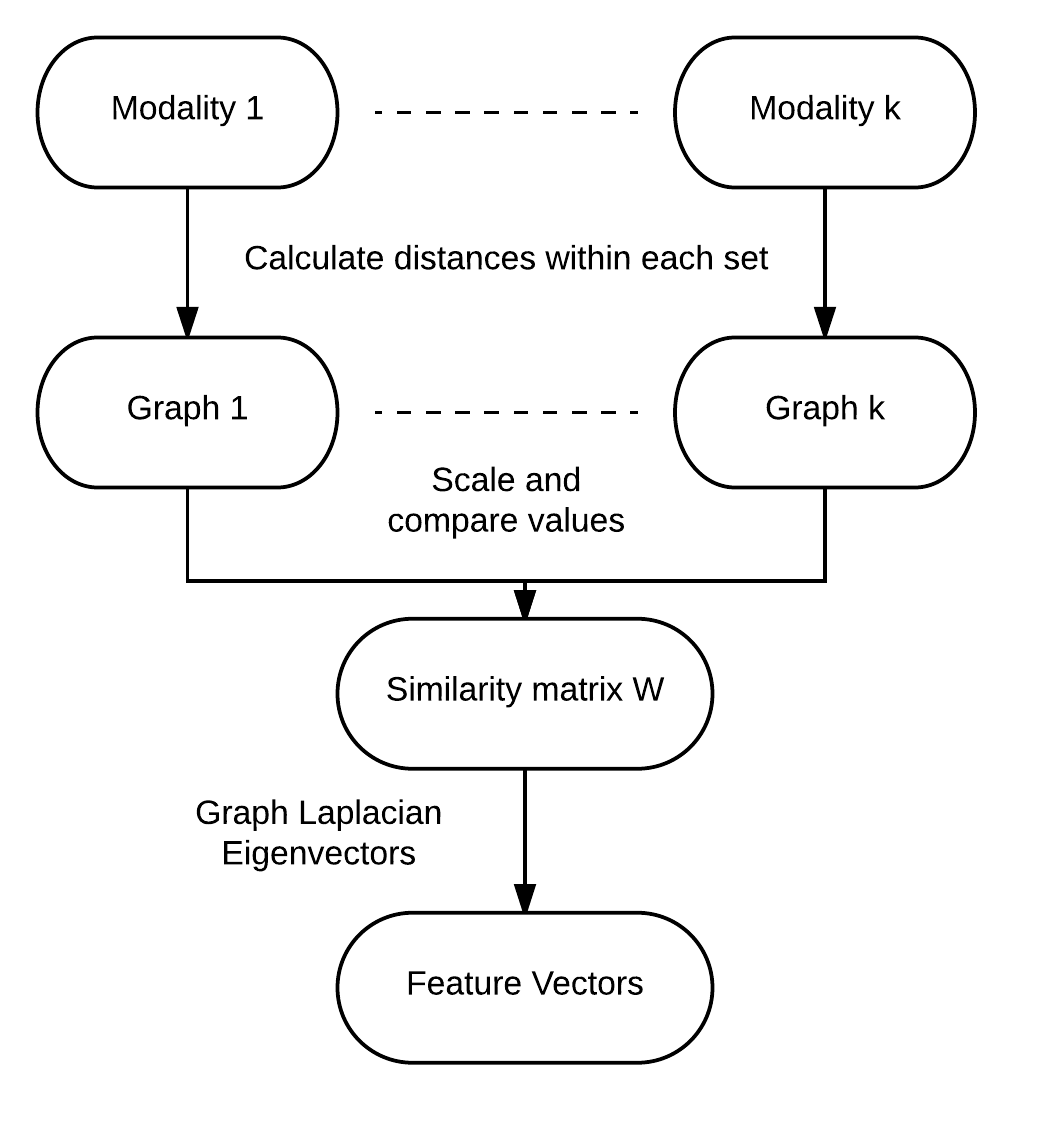
\includegraphics[width=\columnwidth]{./Images/flowchart.png}
  \caption{The Method}
  \label{fig:flowchart}
\end{figure}

% ----------------------------------------- Introduction from 1-15-2017,
% outdated now ----------------------------------------- With the increasing
% availibility of data we often come upon multiple datasets, derived from
% different sources, that describe the same object or phenomenon. These are
% called \emph{multimodal datasets}, and a proper treatment of such sets
% requires more than analyzing each set individually. One common practice is to
% define maps from each set into a common latent space, then perform any
% analysis on this common data. ( talk about canonical correlation analysis, and
% maybe look up parallel factor analysis. I found this in \cite{Lahat15}.) These
% methods aim to find and correlate the redundant information between the
% different sets, however they struggle to identify any information that is
% exclusive to one dataset. Here we present a graph-based approach that aims to
% use the unique information found in each dataset to give a more detailed
% explanation of the source object.

% In this paper we consider the case where each dataset contains the same number
% of elements, and these elements are co-registered (so the $i$-th point in one
% set corresponds to the $i$-th point in another). This situation is often found
% in image processing, where the sets may be images obtained from different
% sources (as is the case in our experimental data), or taken at a different
% time. Call the sets, $X^1,X^2,\ldots,X^m$, with dimensions
% $d_1,d_2,\ldots,d_m$. Let
% $X = (X^1,X^2,\ldots,X^m)\subset \R^{n\times (d_1+\cdots+d_m)}$ be the
% concatenated dataset. Our method creates a latent space $Y$, along with a map
% $X\to Y$. We then use $k$-means to segment the data in $Y$ apply this
% segmentation to $X$. In section \ref{sec:method} we give the general theory
% behind our method, and in \ref{sec:experiment} we show the results of the
% method applied to an Optical/LIDAR dataset.

% ----------------------------------------- A random paragraph from 12/2016. Not
% sure why we have this ----------------------------------------- In this paper
% we address the question of segmentation of multimodal datasets. We provide an
% unsupervised method for data classification Blah blah blah blah. Two datasets,
% $X^s$, $X^t$, that describe the same object. Our goal is to somehow combine
% the sets to form one set $Y$ that blah blah. In the general scenario, $X^s$
% and $X^t$ will often contain redundant information. Previous methods attempt
% to correlate the redundant parts of the two sets, but this often results in a
% overall loss of information, as the data unique to the individual sets isn't
% properly considered. In this paper we aim to emphasize the nonredundant data
% in our creation of $Y$.  Maybe we set up some notation here.

\section{Related Work}
\label{sec:related}

% There is a lot of stuff to add here. For multimodality, some example citations
% are \cite{Tochon2015, Randrianasoa2015, Franek2011, Mitianoudis2007131,
% 4154667, Simone20023, 7325941, Piella2003259, Wattuya2008}. And who knows
% maybe more.

One very simple algorithm for multimodal image fusion is to simply take a
weighted average of the different modes. Unfortunately, this method is often too
naive to produce meaningful results. In many cases there are various objects and
regions that occur in multiple images but with opposite contrast, which would
cancel out in an averaged image. However, this basic idea is still worth
consideration, so long as the blending step is treated with more care. In
\cite{7859418} the authors use structural patch decomposition to perform roughly
the same task, but with much better results, and in \cite{5773085} the authors
address the same problem with probabilistic methods. In each of these cases, the
end product is an image that contains the most relevant features from each
modality. Classical segmentation algorithms can then be performed on this fused
image to create the desired results.

Another common way to fuse images is to transform each modality with some
processing algorithm, then merge the data in the new feature space. In
\cite{Piella2003259} the authors follow this methodology, using a
multiresolution (MR) transformation to process information in each modality. The
benefit of this algorithm is that the transformation is fully invertible,
meaning that once the data has been synthesized in the feature space, the
inverse transformation can be applied to recover the fused image. In
\cite{4154667,Mitianoudis2007131} the authors follow the same overall strategy,
using Independent Component Analysis (ICA) as the initial processing algorithm.

Each of the above methods first fuses the different modalities (into either a
new image, or into a new set of features), then uses this fused data to create a
final segmentation. But another valid method is to instead segment each modality
first, then combine the different classifications into a final result. Both
\cite{Tochon2015} and \cite{Randrianasoa2015} create a hierarchical segmentation
of each modality (a chain of segmentations ranging from very coarse to very
fine), then blend these segmentations using some decision algorithm. A related
field of study is segmentation combination. Given multiple segmentations of the
same image (possibly obtained from different modalities), the goal is to obtain
a consensus segmentation by somehow fusing the different inputs. In
\cite{Franek2011} the authors accomplish this through general ensemble
clustering methods, and in \cite{Wattuya2008} this is done by using
probabilistic methods and random walks.

% \cite{Simone20023} feels like a survey article rather than an actual new
% research thingy. They talk about ``compound classification''. This is
% basically the product method below, but trying to be a little smarter about
% the interaction between the different classes. It's still pretty decision
% level though I think.

In regard to spectral graph theory, these methods have been very successfully
applied to data clustering problems and image segmentation
\cite{1467569,1580491,868688}. Graph-cut algorithms are quite flexible. All that
is required is a well-chosen affinity function to describe the similarity
between different graph nodes. Graph cuts can even be used to minimize a wide
variety of energy functions \cite{1262177}, allowing for the use of unsupervised
\cite{Hu2015,Woodworth13} or semi-supervised methods \cite{Merkurjev13}. The
standard theory behind this is described in \cite{Mohar91}, with a tutorial on
spectral clustering given in \cite{vonLuxburg07}.

\section{The Method}
\label{sec:method}

In this section we explain the theory behind the algorithm. First, in section
\ref{sec:GraphRep} we explain the graph framework used in the later segmentation
steps, including the method for processing the different modalities to create
objects which can be directly compared. We then exhibit two segmentation methods
that we apply to the graph object. The first, \emph{spectral clustering}
\ref{sec:SpecClust}, is an unsupervised method that can be used to quickly
obtain a reasonable set of ``proof-of-concept'' results. The second, \emph{graph
  MBO} \ref{sec:MBO}, is a semisupervised method that more carefully handles the
energy minimization to obtain a stronger final result.

\subsection{Graph Representation} \label{sec:GraphRep}

Let $k$ be the number of input modalities. For each $1\leq i \leq k$, we have a
dataset, which we will label $X^i \subseteq \mathbb{R}^{d_i}$, where $d_i$ is
the dimension of the data. From the co-registration assumption, we have that
each set is the same size.
\begin{align}
  n = \abs{X^1} = \cdots = \abs{X^k}.
\end{align}
And even more, they share a common indexing, which allows us to form the
concatenated dataset
\begin{align}
  X = (X^1,X^2,\ldots,X^k)\subseteq \R^{n\times (d_1+\cdots+d_k)}.
\end{align}
We represent $X$ using an undirected graph $G = (V,E)$. The nodes $v_i\in V$ of
the graph correspond to elements of $X$, and we give each edge $e_{ij}$ a
\emph{weight} $w_{ij}\geq 0$ representing the similarity between nodes
$v_i, v_j$, where large weights correspond to similar nodes, and small weights
to dissimilar nodes. This gives rise to a symmetric \emph{similarity matrix}
(also called a \emph{weight matrix})
\[W = \left(w_{ij}\right)_{i,j=1}^n.\] There are many different notions of
``similarity'' in the literature, and each has its own merits. One common
similarity measure uses a Radial Basis Function
\begin{align}
  w_{ij} = \text{exp}\left(-\text{dist}\left(v_i,v_j\right)^2 / \sigma \right),
\end{align}
where $\sigma$ is a scaling parameter. However, this requires defining a notion
of distance between two graph nodes. In this work, we create such a distance
measure by considering distances between points in each individual modality, as
is explained below.

\subsubsection{Multimodal Edge Weights} \label{sec:Weights}

To calculate the weight matrix $W$, we first scale the sets $X^1, \ldots, X^k$
to make distances in each set comparable. Let
$X = (X^1, \ldots, X^k) \subseteq \R^{n\times (d_1+\cdots+d_k)}$ be the
concatenated dataset. Then for $\ell = 1,\ldots,k$ define the scaling factor
\begin{align}
  \lambda_\ell = \text{stdev}\left(\norm{x_i^\ell-x_j^\ell}\; ;\;1\leq i,j \leq n\right)
\end{align}
For a graph node $x\in X$, we define
\begin{align} \label{eqn:MultimodalEdgeWeights}
  \norm{x} = \max\left( \frac{\norm{x^1}}{\lambda_1},\cdots,
  \frac{\norm{x^k}}{\lambda_k}\right).
\end{align}
Then define the weight matrix $W = \left(w_{ij}\right)_{1\leq i,j \leq n}$ by
\begin{align}
  w_{ij} = \text{exp}\left(-\norm{x_i - x_j}\right).
\end{align}

Note that the $\norm{\cdot}$ defined above is a norm in the formal sense on the
concatenated dataset $X$. The purpose of choosing this specific norm is to
emphasize the unique information that each dataset brings. By using the maximum
of all distances (i.e. the minimum of all similarities) two data points
$x_i,x_j$ are considered similar only when they are similar in every
dataset. For example, in figure \ref{fig:DFCfig1} the gray road and the gray
rooftops are considered very similar in the RGB modality, but quite different in
the lidar modality. Therefore, under this norm the two areas will be given a low
similarity score, as desired.

With any graph-based method, the choice of graph weights is always one of the leading concerns. For this reason, we have studied several different variations of equation \ref{eqn:MultimodalEdgeWeights}, and we present our results in the appendix \ref{sec:WeightsProof}.

\subsubsection{The Graph Laplacian}\label{sec:GraphLaplacian}

Once we have created the weights, we define the \emph{normalized graph
  Laplacian}.  For each node $v_i\in V$, define the \emph{degree} of the node
\begin{align}
  d_i = \sum_j w_{ij}.
\end{align}
Intuitively, the degree represents the strength of a node. Let $D$ be the
diagonal matrix with $d_i$ as the $i$-th diagonal entry. We then define the
\emph{normalized graph Laplacian}
\begin{align}
  L_{sym} = I - D^{-1/2}WD^{-1/2}.
\end{align}
For a thorough explanation of the properties of the graph Laplacian, see
\cite{Mohar91}. In this paper, we will use the connection between the graph
Laplacian and the graph min-cut problem, as explained below.

\subsection{Spectral Clustering}\label{sec:SpecClust}

To implement the first segmentation method, \emph{spectral clustering}, we
rephrase the data clustering problem as a graph-cut-minimization problem of the
similarity matrix $W$. A more detailed survey of the theory can be found in
\cite{vonLuxburg07}. Here we state only the results necessary to implement the
algorithm.

Given a partition of $V$ into subsets $A_1,A_2,\ldots,A_m$, we define the
\emph{graph N-cut}
\begin{align}
  \text{NCut}(A_1,\ldots,A_m) = \frac{1}{2}\sum_{i=1}^m
  \frac{W(A_i,A_i^c)}{vol(A_i)}.
\end{align}
Where
\begin{align}W(A,B) &= \sum_{i\in A, j\in B}w_{ij},\\
  vol(A_i) &= \sum_{i\in A,j\in A}w_{ij} = W(A,A).
\end{align}
Heuristically, minimizing the $N$-cut serves to minimize the connection between
distinct $A_i, A_j$, while still ensuring that each set is of a reasonable
size. Without the $vol(A_i)$ term, the optimal solution often contains one large
set and $m-1$ small sets.

Solving the graph min-cut problem is equivalent to finding an $n \times m$
indicator matrix $u$, where
\begin{align}
  \label{eqn:indicatorMatrix}
  u_{ij} = \begin{cases} 1 & \text{ if } x_i \in A_j \\ 0 & \text{ else}
  \end{cases}.
\end{align}
Here the columns of $u$ correspond to the $m$ different classes. Each row of $u$
will contain a single $1$, which represents the class given to that data point.
It has been shown in \cite{Goldschmidt94} that explicitly solving this problem
is an $O(\abs{V}^{m^2})$ process. As this is infeasible in most cases, we
instead introduce an approximation of the graph min-cut problem that we will
solve using the graph Laplacian. The main tool here is the following fact
(proven in \cite{vonLuxburg07}).
\begin{fact}
  For a given graph-cut $A_1,\ldots,A_m$, define $u$ as above, then
  \begin{align}
    \text{NCut}(A_1,\ldots,A_m) = \text{Tr}\left(u^T L_{sym} u\right).
  \end{align}
\end{fact}
As explained above, it is infeasible to find the $u$ that minimizes the
$N$-Cut. Instead we relax the problem to allow $u$ to be an arbitrary orthogonal
matrix. That is, we find
\begin{align}
  \text{argmin}_{u\in \R^{n\times m}} \text{Tr}\left(u^T L_{sym} u\right)\;\text{
  where }u^Tu=I.
\end{align}
As $L_{sym}$ is symmetric and $u$ is orthogonal, this problem is solved by
choosing $u$ to be the matrix containing the $m$ eigenvectors of $L_{sym}$
corresponding to the $m$ smallest eigenvalues. Using the eigenvectors $u$ we
define a map $X \to \R^m$. For each graph node $x_i\in X$ we get a vector
$y_i\in\mathbb{R}^m$ given by the $i$-th row of $u$. These $y_i$ give the
solution to the relaxed min-cut problem, and as such can be thought of as
features extracted from the original dataset $X$.

To obtain a solution to the original min-cut problem, we then implement some
classification algorithm on the $y_i$. Specifically, for spectral clustering we
use $k$-means on the eigenvectors $u$ to create a final classification into $m$
classes. Although $k$-means is unlikely to give an optimal classification, it is
quite easy to implement, and the final results are strong enough to give a
proof-of-concept.

Note that the eigenvectors $u$ found above are useful for many more purposes
than just spectral clustering. In \ref{sec:experiment} we display some
eigenvectors, and show they can be used to recognize objects in
images. Furthermore, in \ref{sec:MBO}, we will use these same eigenvectors as
part of the MBO algorithm.

\subsection{Semisupervised Graph MBO}\label{sec:MBO}

% \cite{Meng17,Hu2015,Merkurjev13} Notation: let $N = \abs{X}$, $m = $ number of
% classes. We'll keep track of our classification via an $N\times m$
% \emph{assigment matrix} $u$. Entry $(i,j)$ of $u$ stores the probability that
% element $x_i \in X$ belongs in class $j$. The final output matrix will contain
% exactly one $1$ in each row (the rest are zero), but in the intermediate steps
% it can be anything that sums to one. Also, we like to label the $i$-th row of
% $u$ as $u_i$ for notational convenience.

In this section we describe how to use eigenvectors of the graph Laplacian to
segment data in a semisupervised setting. By ``semisupervised'', we mean that
the final classification of a small amount of data points (roughly 5\% of all
data) is used as an input to the algorithm. Following the example set in
\cite{Garcia2014,Merkurjev13,MERKURJEV201429}, we formulate the problem as a
minimization of the Ginzburg-Landau functional.

For the definition of the energy function, we use an $n \times m$ assignment
matrix $u$, similar to the $u$ in (\ref{eqn:indicatorMatrix}). For intermediate steps
of the algorithm, we require that
\begin{align}
  u_{ij} \geq 0 \quad \forall i,j \\
  \sum_{j=1}^m u_{ij} = 1.
\end{align}
Heuristically, the value $u_{ij}$ represents the probability that element $x_i$
will be classified into class $j$. The final output of the algorithm will be a
matrix $u$ where each value is either $0$ or $1$. For notational convenience we
let $u_i$ represent the $i$-th row of $u$. With this notation, we define the
energy function
\begin{align}\label{eqn:GinzburgLandauEnergy}
  E(u) &= \epsilon \cdot \text{Tr}\left(u^TL_{sym} u\right) \nonumber \\
       &+ \frac{1}{\epsilon}\sum_i W(u_i) \nonumber \\
       &+ \sum_i \frac{\mu}{2}\lambda(x_i)\norm{u_i - \hat{u}_i}^2_{L_2}.
\end{align}
The first term of (\ref{eqn:GinzburgLandauEnergy}) is Dirichlet Energy, similar
to \ref{sec:SpecClust}. The second term is the multiwell potential
\begin{align}
  W(u_i) = \prod_{k=1}^{m}\frac{1}{4}\norm{u_i - e_k}_{L_1}^2,
\end{align}
where $e_k$ is the $k$-th standard basis vector. These two terms together
produce an approximation of the classical real Ginzburg-Landau functional, and
it has been shown in \cite{gennip2012} that they converge to the (graph)
total-variation norm as $\epsilon \to 0$. The last term includes the fidelity,
where $\hat{u}$ represents the semisupervised input,
\begin{align}
  \lambda(x_i) = \begin{cases} 1 \quad \text{if $x_i$ is part of fidelity input}\\
    0 \quad
    \text{else}
  \end{cases},
\end{align}
and $\mu$ is a tuning parameter.

The gradient descent update associated to this energy is given by
\begin{align}
  \frac{\pd u}{\pd t} = -\epsilon L_{sym} u - \frac{1}{\ep}W^{'}(u) - \mu\lambda(x)(u-\hat{u}).
\end{align}
Similar to \cite{Merkurjev13,Garcia2014,Meng17}, we propose to minimize this via
an MBO algorithm. If $u^{n}$ represents the $n$-th iterate, then to calculate
$u^{n+1}$ we first diffuse
\begin{align}\label{eqn:diffusion}
  \frac{u^{n+\frac{1}{2}}-u^n}{dt} = -L_{sym} u^n - \mu \lambda(x) (u^n - \hat{u}).
\end{align}
Then threshold each row
\begin{align}\label{eqn:threshold}
  u_i^{n+1} = e_r \quad \text{where }r = \text{argmax}_ju_{ij}^{n+\frac{1}{2}}.
\end{align}
This method effectively splits the energy into two parts and minimizes each
alternatively. The diffusion step (\ref{eqn:diffusion}) handles the
semisupervised Dirichlet Energy (terms 1 and 3 in
(\ref{eqn:GinzburgLandauEnergy})), and the thresholding minimizes the potential
function $W$ (term 2 in (\ref{eqn:GinzburgLandauEnergy})). The stopping
criterion for this algorithm is based on the difference between two consecutive
iterates $u^n,u^{n+1}$. In section \ref{sec:experiment}, we stop the algorithm
when $u^n$ and $u^{n+1}$ agree on 99.99\% of data points.

The diffusion calculation can be done very efficiently by using the
eigendecomposition of $L_{sym}$ (the feature vectors described in
\ref{sec:SpecClust}). If we write
\begin{align}\label{eqn:GLeigendecomposition}
  L_{sym} = X\Lambda X^T
\end{align}
and change coordinates
\begin{align}
  u^n = Xa^n \\
  \mu \lambda(x)(u^n - \hat{u}) = Xd^n
\end{align}
then the diffusion step reduces to solving for coefficients
\begin{align}
  a_k^{n+1} = (1 - dt \cdot \lambda_k)\cdot a_k^n - dt\cdot d_k^n.
\end{align}
where $\lambda_k$ is the $k$-th eigenvalue of $L_{sym}$, in ascending order.

In practice, only a small number of leading eigenvectors and eigenvalues need to
be calculated in order to achieve good accuracy. Therefore, in the
eigendecomposition \ref{eqn:GLeigendecomposition}, we choose a number of
eigenvectors to use, and truncate $X$ to a rectangular matrix. This
significantly improves the speed of the algorithm. Furthermore, in section
\ref{sec:Nystrom}, we discuss how to approximate the leading eigenvectors of
$L_{sym}$ without calculating the full $n \times n$ matrix.

\subsection{Nystr\"{o}m Extension}\label{sec:Nystrom}
Calculating the full graph Laplacian is computationally intensive, as the matrix
contains $n^2$ entries. Instead we use Nystr\"{o}m's extension to find
approximate eigenvalues and eigenvectors with a heavily reduced computation
time. See \cite{Fowlkes04, Merkurjev13, Woodworth13} for a more complete
discussion of this method.

Let $X$ denote the set of nodes of the complete weighted graph. We choose a
subset $A\subset X$ of ``landmark nodes'', and have $B$ its complement. Up to a
permutation of nodes, we can write the weight matrix as
\begin{align}
  W = \begin{pmatrix} W_{AA} & W_{AB} \\ W_{BA} & W_{BB}
  \end{pmatrix},
\end{align}
where the matrix $W_{AB} = W_{BA}^T$ consists of weights between nodes in $A$
and nodes in $B$, $W_{AA}$ consists of weights between pairs of nodes in $A$,
and $W_{BB}$ consists of weights between pairs of nodes in $B$. Nystr\"{o}m's
extension approximates $W$ as
\begin{align}
  W \approx \begin{pmatrix} W_{AA} \\ W_{BA} \end{pmatrix}
  W_{AA}^{-1} \begin{pmatrix} W_{AA} & W_{AB}\end{pmatrix}.
\end{align}
where the error of approximation is determined by how well the rows of of
$W_{AB}$ span the rows of $W_{BB}$. As $W$ is positive semidefinite, we can
write it as a matrix transpose times itself, $W = V^TV$. In \cite{Belongie2002},
the authors show that the Nystr\"{o}m extension estimates the unknown part of
$V$ (corresponding to $W_{BB}$) by orthogonally projecting it into the known
part (corresponding to $W_{AA},W_{AB}$).  This approximation is extremely
useful, as we can use it to avoid calculating $W_{BB}$ entirely. It is in fact
possible to find $\abs{A}$ approximate eigenvectors of $W$ using only the
matrices $W_{AA},W_{AB}$. This results in a significant reduction in computation
time, as we compute and store matrices of size at most $\abs{A}\times\abs{X}$,
rather than $\abs{X}\times\abs{X}$.

In practice, the details of choosing $A$ will not significantly affect the final
performance of the algorithm. Although it is possible to carefully choose the 
``landmark nodes'', in many applications (including this paper) the elements of
$A$ are selected at random from the full set $X$. Assuming the $X$ is not overly
patterned, then it is almost guaranteed that $W_{AA},W_{AB}$ will be full
rank. Furthermore, the amount of landmark nodes $m$ can be chosen to be quite
small without noticeably affecting performance. This makes Nystr\"{o}m's
extension especially useful in application, as very little work is required to
tune the parameters.  In Section \ref{sec:experiment} we use $m = 100$, and
choosing a larger set $A$ does not give a significant change in the error of
approximation.

\section{Experiment}
\label{sec:experiment}

\subsection{Data Fusion Contest 2015 Images}
\label{sec:DFCexperiment}

As a first test for the algorithm, recall the DFC data presented in figure
\ref{fig:DFCfig1}. This set consists of remote sensing images in both the
optical and lidar modalities, and is interesting because of the unique
information brought by each source.

\begin{figure*}[!t]
  \centering \subfloat[Example eigenvector
  1]{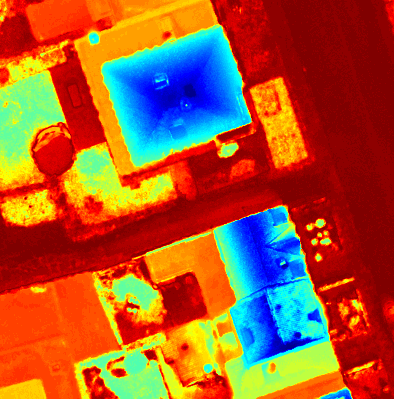
\includegraphics[width=2.5in]{./Images/DFC2015/evec01.png}
    \label{fig:DFCevec1}}%
  \hfil%
  \subfloat[Example eigenvector 2]
  {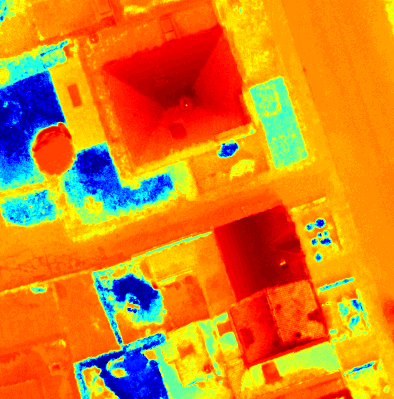
\includegraphics[width=2.5in]{./Images/DFC2015/evec02.png}
    \label{fig:DFCevec2}}%
  \hfil%
  \subfloat[Semisupervised Input]
  {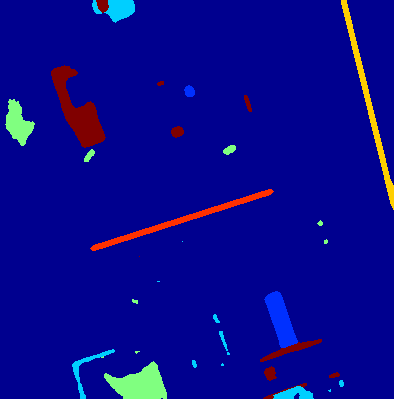
\includegraphics[width=2.5in]{./Images/DFC2015/fidelity.png}
    \label{fig:DFCfidelity}}%
  \hfil%
  \subfloat[MBO
  segmentation]{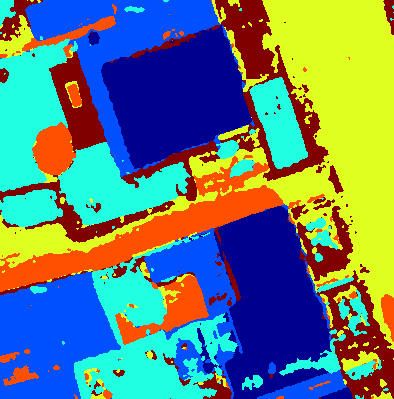
\includegraphics[width=2.5in]{./Images/DFC2015/MBO.png}
    \label{fig:DFCMBO}} %
  \hfil%
  \subfloat[Spectral clustering
  segmentation]{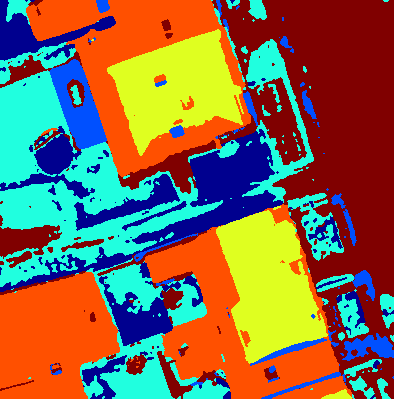
\includegraphics[width=2.5in]{./Images/DFC2015/specClust.png}
    \label{fig:DFCspecClust}}%
  \hfil %
  \subfloat[Direct $k$-means]
  {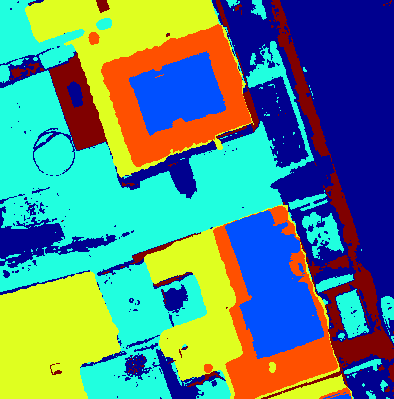
\includegraphics[width=2.5in]{./Images/DFC2015/kmeans.png}
    \label{fig:DFCkmeans}}%
  \caption{DFC features and segmentations}
  \label{fig:DFCfig2}
\end{figure*}

% %%%%%%%%%%%%% May
% %%%%%%%%%%%%% be
% %%%%%%%%%%%%% removed %%%%%%%%%%%%%
% \subfloat[Spectral clustering
% segmentation]{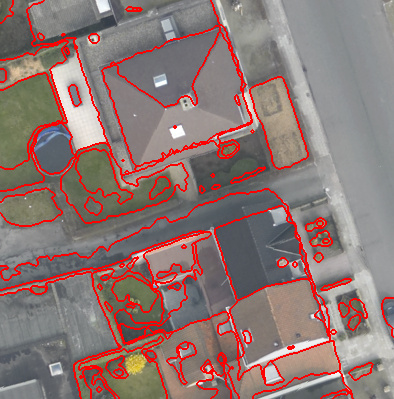
\includegraphics[width=2.5in]{./Images/DFC2015/specClustBorders.png}
% \label{fig:DFCspecClustBorders}}%
% \hfil %
% \subfloat[MBO
% segmentation]{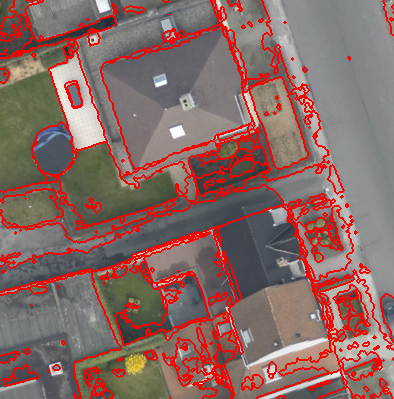
\includegraphics[width=2.5in]{./Images/DFC2015/MBOborders.png}
% \label{fig:DFCkmeans}} %
% %%%%%%%%%%%%%%%%%%%%%%%%%%%%%%%%%%%%%%%%%%%

In figures \ref{fig:DFCevec1}, \ref{fig:DFCevec2}, we show two example
eigenvectors of the graph Laplacian. As explained in \ref{sec:SpecClust}, these
vector can be thought of as feature of the dataset, and looking at them will
give us a rough idea of the final segmentation. Notice how in \ref{fig:DFCevec1}
the dark-gray asphalt is distinct from both the nearby grass (which is at the
same elevation), and the roofs of the buildings (which are a similar
color). This shows at the feature level that the algorithm is successfully using
both the optical and the lidar data when determining what pixels can be
considered similar. Based on this example vector, the classification algorithm
then separates those regions in the final results. One can note the similarities
between each of the example eigenvectors and the final classifications
\ref{fig:DFCspecClust}, \ref{fig:DFCMBO}.

For this image, we choose to segment the data into 6 classes. As the data does
not come with any ground truth attached, the number 6 was chosen based purely on
personal opinion. The classes given in the semisupervised term (fig
\ref{fig:DFCfidelity}) are roughly: tall buildings, mid-level buildings, asphalt
(bright), asphalt (dark), white tiles, and grass. The exact choice of fidelity
pixels was made by either manually choosing locations, or by characteristics of
the data (ex: the 1\% of pixels at highest elevation). Most importantly, these
classes can all be separated using either color or lidar (or both).

As should be expected, the spectral clustering method (fig
\ref{fig:DFCspecClust}) does not select exactly the same 6 classes that we have manually
identified. As this algorithm is unsupervised, there is no way of encoding our
human preference into the method. Therefore, the choice of exactly how to divide
the different groups of pixels is made in accordance with just the graph min cut
energy. In the end, this algorithm can still pick out the major features of the
dataset, but the specific decisions of exactly which classes to combine and
which to separate does not agree with our human intuition. By instead using a
semisupervised algorithm such as graph MBO (fig \ref{fig:DFCMBO}), we can input
a small amount of information (in this case, 7\% of total pixels) in order to
align the energy minimization with our human expectations. Therefore, the final
result aligns quite well with initial expectations.

When choosing the exact parameters for the algorithm, there are several factors
to consider. First, the diffusion step should be stable, which occurs when $dt$
and $\mu$ are relatively small. Second, the final result should agree with the
semisupervised input (fig \ref{fig:DFCfidelity}), which occurs when $\mu$ is
relatively large. Third, the runtime should not be too long, which occurs when
$dt$ is relatively large. Balancing these different goals required multiple
trial runs of the code. In this particular example we use parameters
$dt = 0.1, \mu = 10^4$.

For comparison, we also show the results of a more naive algorithm.  In figure
\ref{fig:DFCkmeans} we apply $k$-means directly to the concatenated
(4-dimensional) dataset, without any preprocessing. As can be seen from the
result, a direct application of $k$-means is not well suited towards handling
information from disparate sources. In this particular example, the segmentation
overvalues the information from the lidar modality, and therefore overclassifies
the buildings based on height. This, in turn, results in a poor classification
of the different ground-level features, as the RGB information is not well-used.

%%%%%%%%%%%%%% May be removed %%%%%%%%%%%%%
% For comparison, we show the results of two other classification methods in
% figures \ref{fig:DFCproduct} and \ref{fig:DFCkmeans}. The product method in
% \ref{fig:DFCproduct} is a basic decision-level data fusion method. Here we use
% similar graph methods to segment each individual modality, then take the
% product of these classifications to create the final segmentation (in the
% product, two pixels lie in the same class iff they agree in both of the
% individual segmentations). This method is generally slower, as it requires
% running the segmentation process twice, and the results range from slightly
% worse to much worse than the algorithm, depending on the data. In figure
% \ref{fig:DFCkmeans} we apply kmeans to the original dataset.

% To give some quantitative comparisons, we must first define an error
% metric. Unfortunately, for a given segmentation of an image computing the
% graph-cut error as described in \ref{sec:SpecClust} is an $O(n^2)$
% calculation, and requires the full weight matrix $W$. To avoid this, we
% instead measure the error of segmentation by how the data
% $X = (X^1,\ldots,X^k) \subset \R^{n\times (d_1+\cdots+d_k)}$ varies within
% each class. More explicitly, we use the metric:
% % max method.
% \begin{align}
%   \text{Error} = \frac{1}{n}\sum_{\text{classes }\cC}\sum_{x\in \cC}\norm{x - \text{mean}\left(y\in \cC\right)}.
% \end{align}
% Error here: my method is 0.4072 union method is 0.4377 2-norm method is 0.4140
% optical only is 0.8338 lidar only is 0.7504
%
%
% std method. I think I did the math wrong here.
% \begin{align}
%   \text{Error}
%   =
%   \sum_{\text{classes
%   % }\cC}\text{std}\left(x
%     \in
%     \cC\right).
% \end{align}
% I don't have data for this method saved, which is probably dumb of me.  Where
% the norm $\norm{\cdot}$ is the same as defined in \ref{sec:Weights}. The
% results for each of the sample methods are given in table
% \ref{table:DFCExperimentQuantitative}. Most of the experimental methods are
% pictured above, with the exception of the multimodal method with weights drawn
% from the standard 2-norm. This is a slight variation on the method explained
% in \ref{sec:method}, where instead of the norm used in \ref{sec:Weights}, we
% define
% \begin{align} \label{eqn:2norm} \norm{x} =
%   \sqrt{\frac{\norm{x^1}^2}{\lambda_1} + \cdots +
%   \frac{\norm{x^k}^2}{\lambda_k}},
% \end{align}
% and create the weight matrix using this metric. Interestingly, the change in
% norm causes very little change in the final segmentation. The runtimes here
% are taken from a personal laptop, and should only be used for relative
% comparison within this paper.
% \begin{table} [htb]
%   \centering
%   \begin{tabular}{l l l}
%     \textbf{Method} & \textbf{Error} & \textbf{Runtime}\\
%     The method \ref{fig:DFCsegmentation} & 0.40 & TODO: \\
%     The method with 2-norm (eqn \ref{eqn:2norm}) & 0.41 & need \\
%     Product method \ref{fig:DFCproduct} & 0.43 & to \\
%     Graph cut on optical only \ref{fig:DFCopticalOnly} & 0.83 & update \\
%     Graph cut on lidar only \ref{fig:DFClidarOnly} & 0.75 & this \\
%     K-means on original data \ref{fig:DFCkmeans} & 0.75 & table \\
%   \end{tabular}
%   \caption{DFC quantitative comparisons}
%   \label{table:DFCExperimentQuantitative}
% \end{table}


\subsection{Umbrella Data}
\label{sec:UmbrellaExperiment}

\begin{figure*}[!t]
  \centering \subfloat[Umbrella optical
  data]{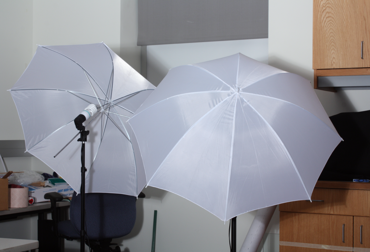
\includegraphics[width=1.75in]{./Images/Umbrella/optical.png}%
    \label{fig:UmbrellaOptical}} \hfil \subfloat[Umbrella lidar
  data]{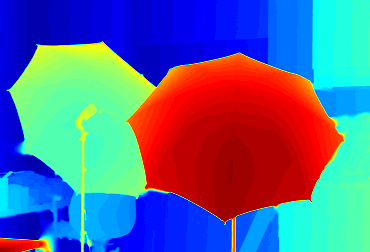
\includegraphics[width=1.75in]{./Images/Umbrella/lidarColor.png}%
    \label{fig:UmbrellaLidar}} \hfil \subfloat[Semisupervised Input]
  {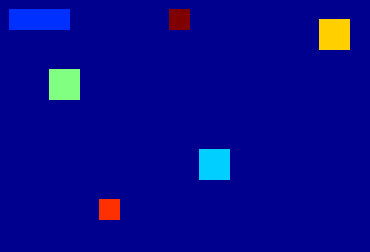
\includegraphics[width=1.75in]{./Images/Umbrella/fidelity.png}%
    \label{fig:UmbrellaFidelity}} \hfil \subfloat[Example eigenvector
  1]{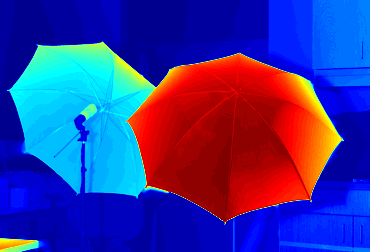
\includegraphics[width=1.75in]{./Images/Umbrella/evec01.png}%
    \label{fig:UmbrellaEvec1}} \hfil \subfloat[Example eigenvector 2]%
  {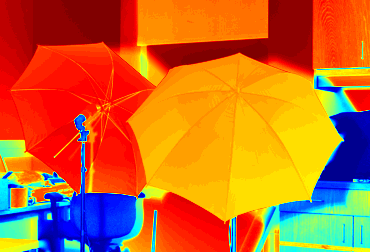
\includegraphics[width=1.75in]{./Images/Umbrella/evec02.png}%
    \label{fig:UmbrellaEvec2}} \hfil \subfloat[Example eigenvector 3]%
  {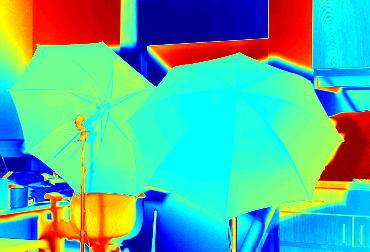
\includegraphics[width=1.75in]{./Images/Umbrella/evec04.png}%
    \label{fig:UmbrellaEvec3}} \hfil \subfloat[Spectral clustering
  segmentation]{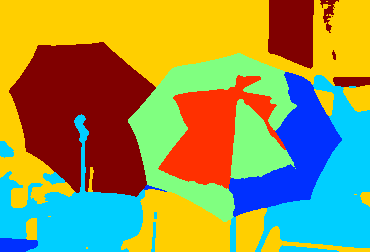
\includegraphics[width=1.75in]{./Images/Umbrella/specClust.png}%
    \label{fig:UmbrellaSpecClust}} \hfil \subfloat[MBO
  segmentation]{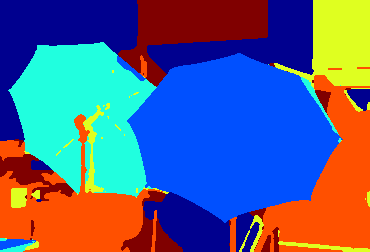
\includegraphics[width=1.75in]{./Images/Umbrella/MBO.png}%
    \label{fig:UmbrellaMBO}} \hfil \subfloat[Direct $k$-means]
  {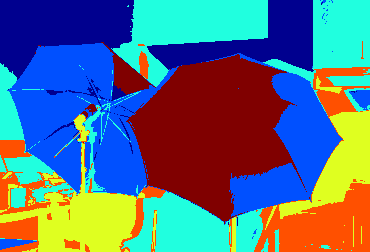
\includegraphics[width=1.75in]{./Images/Umbrella/kmeans.png}%
    \label{fig:Umbrellakmeans}}
  \caption{Umbrella data results}
  \label{fig:Umbrella}
\end{figure*}

In fig \ref{fig:Umbrella} we show the results of the method applied to another
optical/lidar set (found in \cite{Scharstein14}), which we will refer to as the
umbrella data. Similar to the DFC set, the umbrella data serves as a good
example because it cannot be easily analyzed using one modality alone. The
umbrellas and the background walls are nearly the same shade of white, and can
only be distinguished in the lidar data. Meanwhile, the different pieces of the
background all lie at nearly the same depth, and can only be separated by
color. As was the case with the DFC data, the final classifications
\ref{fig:UmbrellaSpecClust}, \ref{fig:UmbrellaMBO} can be understood by looking
at the individual feature vectors. In figure \ref{fig:UmbrellaEvec1}, we see
very clearly the difference the major features of the dataset: the front
umbrella, the back umbrella, and the background wall. Figures
\ref{fig:UmbrellaEvec2}, \ref{fig:UmbrellaEvec3} show more of the small details
of the data, separating the many different background objects.

As was the case with the DFC data, we chose to segment this image into 6 classes
based primarily on personal opinion. The classes represented in the
semisupervised input are: the front umbrella, the back umbrella, the wooden
cabinet in the corner, and various different colors of background objects (fig
\ref{fig:UmbrellaFidelity}). Similar to the results from the DFC dataset, we can
find many major features in the spectral clustering result (fig
\ref{fig:UmbrellaSpecClust}), but the exact details of the classification do not
match our expectations. In particular, the foremost umbrella of this set is
overclassified, which in turn forces the algorithm to combine the background
objects into a small number of classes. In the graph MBO result (fig
\ref{fig:UmbrellaMBO}), we give include the class of 5\% of pixels as part of
the input, and as such the classification fits the original data much more
closely.

In figure \ref{fig:Umbrellakmeans} we again show the result of applying
$k$-means directly to the concatenated dataset. As seen before, this naive
algorithm struggles to make use of all the information present in the different
modalities. In this example, the issue can be seen most clearly in the failure
to separate the two umbrellas. $k$-means succeeds in separating many objects
based on their RGB value, but the fact that the two umbrellas are grouped into
the same class shows that the lidar information is not properly valued.

% %%%%%%%%%%%%% May be removed %%%%%%%%%%%%%
% \begin{table}[htb]
%   \centering
%   \begin{tabular}{l l l}
%     \textbf{Method} & \textbf{Error} & \textbf{Runtime}\\
%     \textbf{Our method} & 0.31 & 9.0s\\
%     Our method with 2-norm & 0.33 & 8.4s\\
%     Product method & 0.51 & 16.6s \\
%     Graph cut on optical only & 0.86 & 8.1s \\
%     Graph cut on lidar only & 0.50 & 6.7s \\ 
%     K-means on original data & 0.52 & 3.1s \\
%   \end{tabular}
%   \caption{Umbrella data quantitative comparisons}
%   \label{table:UmbrellaExperimentQuantitative}
% \end{table}
% %%%%%%%%%%%%% May be removed %%%%%%%%%%%%%

\subsection{Jade Plant Data}

Found in the same paper as the umbrella data \cite{Scharstein14}, we test the
method against another optical/lidar scene of a jade plant, shown in figures
\ref{fig:JadeplantOptical}, \ref{fig:JadeplantLidar}. As with all examples shown
here, there is a large amount of non-redundancy between the two input images. In
particular, in this example the optical image is quite homogeneous, as it is
mostly composed of shades of brown. Therefore, one would expect the addition of
the lidar data to greatly aid the segmentation.

In figures \ref{fig:JadeplantEvec1}, \ref{fig:JadeplantEvec2}, we once again
show a few example eigenvectors extracted from the input data. As before, we can
see in each eigenvector some pieces of the final classifications
\ref{fig:JadeplantSegmentation}, \ref{fig:JadeplantMBO}.
\begin{figure*}[!t]
  \centering \subfloat[Jade plant optical
  data]{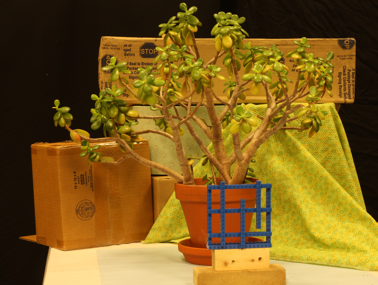
\includegraphics[width=1.75in]{./Images/Jadeplant/optical.png}
    \label{fig:JadeplantOptical}} %
  \hfil%
  \subfloat[Jade plant lidar
  data]{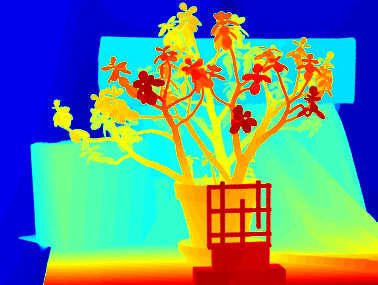
\includegraphics[width=1.75in]{./Images/Jadeplant/lidar.png}
    \label{fig:JadeplantLidar}}%
  \hfil%
  \subfloat[Example eigenvector
  1]{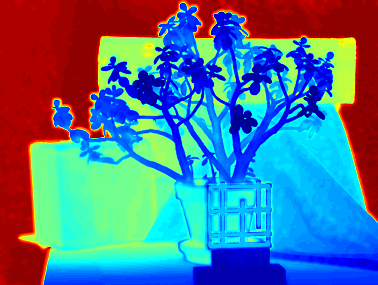
\includegraphics[width=1.75in]{./Images/Jadeplant/evec01.png}%
    \label{fig:JadeplantEvec1}} \hfil \subfloat[Example eigenvector
  2]{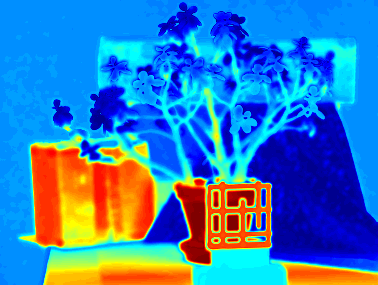
\includegraphics[width=1.75in]{./Images/Jadeplant/evec03.png}%
    \label{fig:JadeplantEvec2}} \hfil \subfloat[Spectral clustering
  segmentation]
  {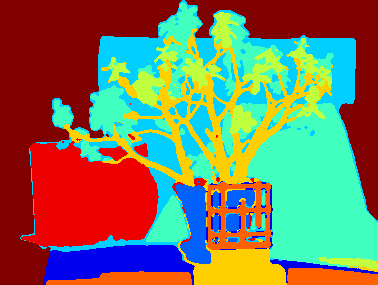
\includegraphics[width=1.75in]{./Images/Jadeplant/specClust.png}%
    \label{fig:JadeplantSegmentation}} \hfil \subfloat[MBO segmentation]
  {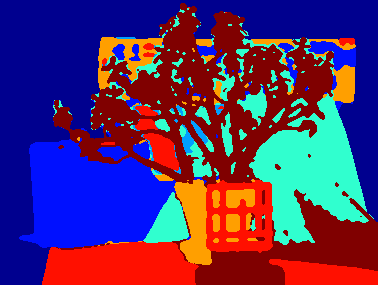
\includegraphics[width=1.75in]{./Images/Jadeplant/MBO.png}%
    \label{fig:JadeplantMBO}}
  \caption{Jade plant data results}
  \label{fig:Jadeplant}
\end{figure*}

\section{Conclusions}
\label{sec:conclusions}

In conclusion, graph-based methods provide a straightforward and flexible method
of combining information from multiple datasets. By considering the similarity
between points in each individual dataset, we reduce the information from each
modality into something more directly comparable. This in turn gives us a model
that is more data-driven, using the information obtained from each modality
without needing to know the details about the source from which the data was
captured. Therefore the same algorithm could be applied in many different
scenarios, with different types of data.

Once we have calculated and compared the different weight matrices, we can then
create the graph Laplacian of the data and extract features in the form of
eigenvectors. These features can then be used as part of many different
data-segmentation algorithms. For this paper, we use $k$-means on the
eigenvectors as a simple proof-of-concept, and graph MBO as a more in-depth
approach. The main computational bottleneck is in calculation of the
eigenvectors. Once we have these, there are many different viable
classifications in the literature.

A future area of interest is to further generalize the method by removing or
weakening the co-registration assumption. This segmentation algorithm only
considers cases where the two images are of the same underlying scene, where
pixels correspond exactly between images. But it would be interesting, for
example, to process two images taken from different angles. In image processing
problems, co-registration is usually a reasonable assumption. However, removing
this assumption would allow this algorithm to be applied to data fusion problems
across a huge number of fields.

% TODO: Add a bit about \cite{lahat:hal-01062366} talks about how all the cool
% data fusion algorithms available right now are very specialized. People are
% looking for a method that is data driven and doesn't depend on any models. We
% want to do that.  This particular project doesn't do a perfect job but it's
% still a good start along the right path.

\section{Acknowledgments}\label{sec:Acknowledgements}

This work was supported by NSF grant DMS-1118971, ONR grant N00014-16-1-2119,
NSF grant DMS-1417674, European Research Council (Grant no. 320684 - CHESS
project), and CNRS (Grant no. PICS-USA 263484)

\appendix
\section{Appendix: Choice of Norm to Combine Modalities}\label{sec:WeightsProof}

In section \ref{sec:Weights}, we create our multimodal edge weights by choosing the largest distance found throughout the different modalities. However, we could replace the $\max$ in equation \ref{eqn:MultimodalEdgeWeights} with a large number of different options, the easiest of which is to use a different $L^p$ norm (thinking of $\max$ as the $L^\infty$ norm). The question then arises, if we choose a different $L^p$ norm, what difference should we expect in the final result? In this section we aim to answer this question, both on the level of heuristics, as well as with some more concrete observations.

The most obvious heuristic is that choosing a large $p$ causes the edge weights to be heavily affected by individual outliers among modalities, whereas choosing a small $p$ will provide more of an averaging effect over all the modalities. In this paper we choose to use the $L^\infty$ norm because we expect each modality to separate some, but not all, of the objects. In other words, we believe that two pixels should be considered similar only if they are similar in every modality, and a single diffrence shown across all modalities is worth our consideration. However, for a different application - for example, when working with noisy data - a different choice of $p$ could create a better final result.

These heuristics give an idea of the quality of difference between two choices of norms, but it is also desirable to understand the quantity of difference. If we change our choice of $p$ norm, how much change can we expect in the graph weights, and in the resulting graph cut? Unsurprisingly, this answer is highly dependent on the number of modalities, as for $1 \leq p < q \leq \infty$ we have the inequality
\begin{align}
  \norm{x}_p \leq \norm{x}_q \leq n^{1/p - 1/q}\norm{x}_p,
\end{align}
where $n$ is the dimension of the vector $x$. So when working with relatively few modalities, a different choice of $p$ norm will not make a large difference in the distance between points (and therefore the graph weights). However, as the number of modalities increases, it is possible to have large differences in the graph weights as a result of changing $p$. We formalize this statement in the theorem below.

\subsection{Theorem and Proof}

We begin with some notation to simplify the statement of the theorem. Suppose we have $n$ points $x_1,\ldots,x_n$ in some $\R$-space. We're interested in distances between points in different norms. So let
\begin{align}
  d_{ij}^p &= \norm{x_i - x_j}_p \\
  D^p &= \left\{d_{ij}^p \,:\, 1\leq i < j \leq n\right\}
\end{align}
In other words, for each choice of $p$ there are $n \choose 2$ values that we're interested in. More specifically, we are interested in the ordering under $\leq$ for each of these sets $D^p$, as the graph weights are depend on the relative size of the different $d_{ij}^p$ rather than on the absolute size. As we show below, if the ambient dimension is large enough it is possible to simultaneously control the orderings in more than one $D^p$ by properly choosing the $x_1,\ldots,x_n$.

\begin{theorem} For any $1 \leq p < q \leq \infty$, it is possible to choose the $x_1,\ldots,x_n \in \R^n$ to simultaneously produce any arbitrary ordering under $\leq$ on both $D^p$ and $D^q$.
\end{theorem}
\begin{proof}
  It suffices to give a proof for the case $p=1, q=\infty$, as the $L^p$ norm on $\R^n$ is a decreasing function of $p$, and therefore any inequalities in the case $p = 1, q = \infty$ will hold in the general case $1 \leq p < q \leq \infty$ as well.

  To construct the $x_1,\ldots,x_n$ that produce the distances we desire, we first begin with the standard basis vectors
  \begin{align}
  x_i = e_i \quad 1\leq i \leq n
  \end{align}
  then proceed to make small edits to the $x_i$ to achieve the desired order. Note that before making any changes, $d_{ij}^1 = 2, d_{ij}^\infty = 1$ for all $i,j$. To properly order the $L^1$ distances, we makes the following type of adjustment where necessary:
  \begin{align}\label{eqn:move1}
    x_i^{new} = x_i^{old} + \epsilon\cdot e_j\quad\text{for some }\epsilon < 1,
  \end{align}
  as pictured in figure \ref{fig:move1}. This decreases $d_{ij}^1$ by $\epsilon$, increases $d_{i\ell}^1$ by $\epsilon$ for $\ell \neq j$, and does not affect $d_{\ell k}^\infty$ for any $\ell, k$.

  Once the $L^1$ distances are properly set, we can fix the $L^\infty$ distances as follows:
  \begin{align}\label{eqn:move2}
    x_i^{new} = x_i^{old} + \epsilon\cdot e_j - \epsilon\cdot e_i \quad\text{for some }\epsilon < 1,
  \end{align}
  as pictured in figure \ref{fig:move2}. This decreases $d_{ij}^1$ by $2\cdot\epsilon$, decreases $d_{ij}^\infty$ by $\epsilon$, and does not affect $d_{\ell k}^\infty$ for any $\ell, k$.

  Given these two possible moves, it's relatively simple to achieve the desired ordering of distances by using progressively decreasing values of epsilon. At each step one can choose epsilon sufficiently small so that the changes from the previous steps are not affected. For example, if one could use $\epsilon = 2^{-k}$ for the $k$th move.
  
  \begin{figure}
    \centering
    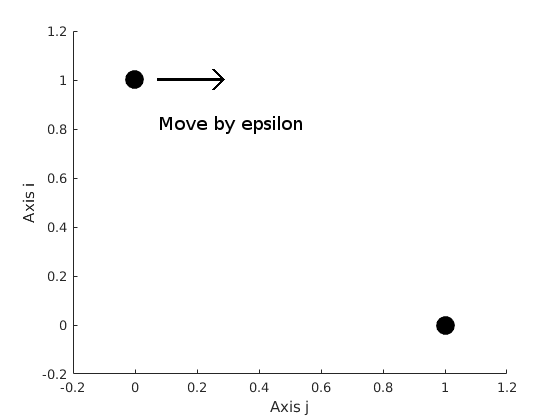
\includegraphics[width = 0.9\linewidth]{./Images/WeightTheory/move1.png}
    \caption{Move 1}
    \label{fig:move1}
  \end{figure}
  \begin{figure}
    \centering
    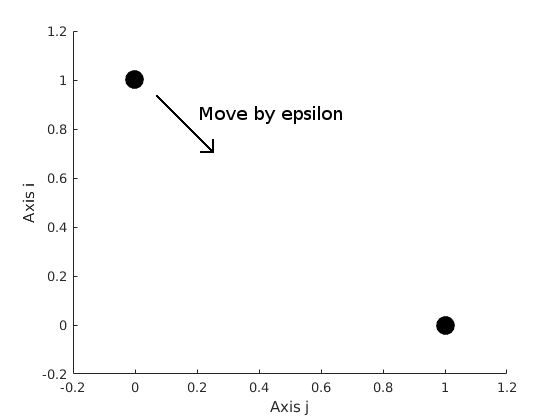
\includegraphics[width = 0.9\linewidth]{./Images/WeightTheory/move2.png}
    \caption{Move 2}
    \label{fig:move2}
  \end{figure}
\end{proof}

\bibliographystyle{unsrt} \bibliography{../../BibTex/research}

\end{document}
